\documentclass[letterpaper,12pt,fleqn]{article}
\usepackage{matharticle}
\usepackage{tikz}
\pagestyle{empty}
\begin{document}
\section*{Math-42 Final Study Guide}

There are 30 questions, most with multiple parts.  That gives you an average of about 1 minute per question/part,
so don't get stalled on any one question.  Here is a rundown of the questions.

\begin{enumerate}[left=0in]
\item This question is about relations and what makes a relation a function.  Recall that for two sets \(A\) and
  \(B\), a relation between \(A\) and \(B\) is simply a subset of their cross-product: \(R\subseteq A\times B\).
  A function is a relation where everything in the domain \(A\) is used and each value in the domain maps to
  exactly one value in the codomain \(B\).

  You are given two sets and a description of various relations.  Your job is to build a bubble diagram that
  demonstrates what is related to what and then to decide which of the relations are also functions.

  For example, let \(A=\set{1,2,3}\) and \(B=\set{2,5}\).  Let \(R\) be the relation defined by
  \((x,y)\in R\) iff \(x+y\) is even.  So you would construct a bubble chart that looks like this:

  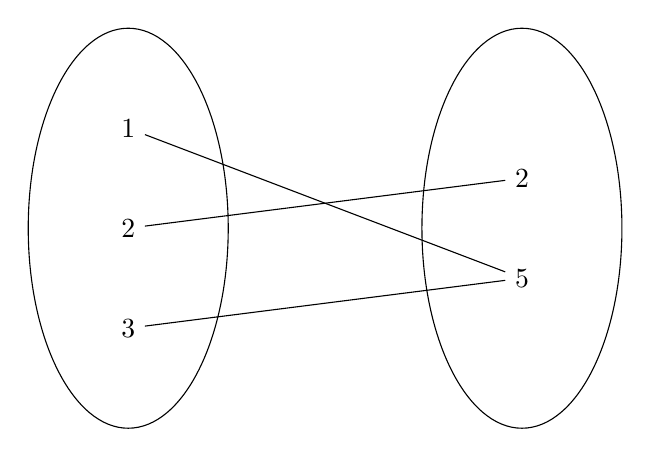
\begin{tikzpicture}
    \draw (0,0) ellipse (0.5in and 1in);
    \draw (5,0) ellipse (0.5in and 1in);
    \node (A1) at (0,0.5in) {1};
    \node (A2) at (0,0) {2};
    \node (A3) at (0,-0.5in) {3};
    \node (B2) at (5,0.25in) {2};
    \node (B5) at (5,-0.25in) {5};
    \draw (A1) -- (B5);
    \draw (A2) -- (B2);
    \draw (A3) -- (B5);
  \end{tikzpicture}

  You would then conclude that this is in fact a function, because each domain value is used and maps to exactly
  one codomain value.

\item This question gives you some statements and asks you to construct compound statements from them.  For
  example:

  \(P\coloneq\) Max is a cat.
  \(Q\coloneq\) Max is black.
  \(R\coloneq\) Max sleeps a lot.

  If you are asked to construct the sentence: ``Max is a cat but he is neither black nor sleeps a lot'' your
  answer would be \(P\land(\lnot Q\land\lnot R)\), or using DeMorgan, \(P\land\lnot(Q\lor R)\).

  Be careful with the construct neither-nor.  This means that both are not true.

\item This question gives a fairly straightforward logic equation and asks you to fill in a truth table.  You
  shouldn't have any problems here.

\item This question demonstrates that only a single counterexample is needed to disprove the universal
  quantifier.  You are given a universally quantified statement and asked to find a counterexample.  If the
  domain is integers, be sure to always try the simple cases like 0 and 1 first.

\item This questions gives you three predicates and asks you to build quantified statements from them, similar
  to the \(x\) loves \(y\) problem.

\item This question gives you are quantified statement and asks you to negate it.  For example, if you were
  asked to negate ``All men are pigs'', your answer would be either ``There exists a man that is not a pig'' or
  ``Some men are not pigs''.

\item This question asks you to negate nested quantifiers, like out limit and continuity definitions that we did
  in class and in the written homework.

\item This question asks you to construct a direct proof related to even and odd integers.  Remember our
  definitions of even and odd.  Also remember the template of a direct proof:
  \begin{enumerate}
  \item Instantiation
  \item Definitions
  \item Inner steps (usually algebra)
  \item Definitions
  \item Generalization (implicit)
  \item Conclusion
  \end{enumerate}
  Webassign gives you some candidate steps that you need to select and then put in the proper order.  I suggest that
  you write the proof first off to the side and then try to construct it using the steps that webassign provides.

\item This question tests your knowledge of the definition of a rational number: to say that \(r\) is a rational
  number means that \(\exists\,p,q\in\Z\) such that \(q\ne0\) and \(r=\frac{p}{q}\).

\item This question tests you knowledge of what it means for one integer to divide a number: to say that
  \(n|m\) means that there exists \(k\in\Z\) such that \(m=kn\).  Be sure to understand the cases when \(n\) or
  \(m\) or both are 0.

\item This question gives you an integer and a divisor and asks you to construct the division algorithm
  expansion.  Be sure that you know how to do this for both positive and negative numbers.

\item This question is another arrange the steps into a proof question, this time regarding the concept of one
  integer dividing another.  (hint: check to see if contradiction or contrapositive is appropriate).

\item You are given a sequence and asked to come up with a closed form for \(a_n\).  This one is not too hard.

\item You are given the recursive form of a sequence (with initial condition) and are asked to determine the
  first four elements of the sequence.  Don't forget the initial condition!

\item This question is a bit harder.  It tests your understanding of the generalized union and intersection.
  You should review this material on pages 140 and 141 of the Rosen text.  A good example is page 145 number 43:

  Let \(A_i=\set{1,2,3,\ldots i}\).  Determine the following:
  \[\bigcup_{i=1}^nA_i=\set{1,2,\ldots n}\]
  \[\bigcap_{i=1}^nA_i=\set{1}\]

\item This question gives you a bunch of 3-set Venn diagrams and some set logic equations.  You need to select
  the regions descrobed by the equations.  For example, if you are given \(A\cap B\), you would check the
  intersecting region.

\item This questions tests you knowledge of the terminology related to functions.  Make sure that you
  understand the terms domain, codomain, range, image, and preimage and given the bubble diagram of a function
  can pick out these various elements.

\item This question is a permutation question.  You are asked for both total possible and total given some
  limiting conditions.  Here is a good example.

  Consider bit strings of length 10.  How many possible are there?  \((2^{10}=1024)\).  How many begin with a '1'
  and end with a '0'?  \((2^8=256)\).

\item This question involves the pigeonhole principle and is of the ``what is the minimum number'' type.  Remember
  that this is controlled by the formula: \(n(r-1)+1\).

\item This question is a committee formation problem.  There are different parts that place different
  constraints on the selection.  For example, given 10 people and you need to form a committee of 5, how many
  possible?  How many possible if 6 men and 4 women and you want a committee of 2 men and 3 women?  What is
  Jim and Jill won't serve together, etc.

\item This is a balls in the urn problem, but you are going to make only 2 selections with no replacement.  You are
  to build a decision tree and answer questions about the various probabilities.  Note that there is no replacement,
  so conditional probabilities come into play here.

\item This is a PIE problem.  Given a range of numbers, you are asked to determine how many are divisible by
  two different numbers and need to calculate the total divisible by both numbers.

\item Your are given a range of numbers and asked how many of those numbers are divisible by some number.  For
  example, if your range is 1 to 100, and you are asked how many integers in that range are divisible by 7, how
  would you do it? floor(100/7)=14.  You are then asked some probability questions based on the results.  For
  example, it you pick a number at random in the range, what is the probability that it is divisible by 7:
  \(\frac{14}{100}=0.14\).

\item This is a sticky-letter problem.  For example, how many ways to arrange the letters in ``first'' assuming
  that the ``ir'' must occur together in that order.

\item You are asked about a sample space of multiple coin flips and the probabilities of various events.

\item A composition problem.  You are given two functions and need to calculate the composition for various domain
  values.  Remember that \((f\circ g)(x)=f(g(x))\).  One of the functions may be mod-related.

\item In this problem you are given some bubble diagrams of functions and are asked to determine whether they are
  injective (one-to-one) or surjective (onto) and why.

\item In this problem you are given a function and asked to determine if it is injective.  Remember the proof
  template: assume \(f(a)=f(b)\) and then show (using algebra) that \(a=b\).

\item This problem asks you to negative a nested quantifier that has a conditional.  Remember how to negate
  a conditional: \(\lnot(p\implies q)\equiv p\land\lnot q\).

\item You are given a proof of a logic equation and you are asked to identify each step per the table on
  page 29.
\end{enumerate}

\end{document}
